\documentclass[a4paper,11pt]{article}
\usepackage{preamble}

\title{Machine Learning Course\\\large{Notebook}}
\author{Mariana Jó}
\date{\today}

\begin{document}
  \maketitle
  \thispagestyle{fancy}


  \section{What is Machine Learning?}
  \begin{itemize}
    \item Definitions of ML \\
    \textit{"A computer program is said to learn from experience E with respect to some class of tasks T and performance measure P, if its performance at tasks in T, as measured by P, improves with experience E."}
    \item Kinds of ML algorithms
  \end{itemize}

  \section{Supervised learning}
  Some definitions:
  \begin{itemize}
    \item Supervised Learning: We give the dataset the "right answers"
    \item Regression: predict continous valued output
    \item Classification: discrete valued output
    \item Support Vector Machines: an algorithm that can deal with an infinite number of features
  \end{itemize}
  \section{Unsupervised learning}
  \textit{"Unsupervised learning allows us to approach problems with little or no idea what our results should look like. We can derive structure from data where we don't necessarily know the effect of the variables. With unsupervised learning there is no feedback based on the prediction results."}
  \begin{itemize}
    \item Clustering: groups things that are somehow similar and/or related
    \item Non-clustering: finds structure. Ex.: cocktail party algorithm.
  \end{itemize}

  \section{Model representation}
  \textbf{Notation:}
  \begin{itemize}
    \item $m=$ Number of training examples
    \item $x=$ "input" variable / features
    \item $y=$ "output" variable / "target" variable
    \item $(x,y)=$ one training example
    \item $\theta=$parameter
  \end{itemize}
  About hypothesis $h$:
  \begin{itemize}
    \item Hypothesis $h$: takes the input $x$ and outputs the estimated value $y$, i.e., $h$ maps from $x$'s to $y$'s.
    \item How do we represent $h$? \\
    We choose an initial choice
    \begin{equation}
    h_\theta (x)=\theta_0 +\theta_1 x  ,
    \label{eq:hypothesis}
    \end{equation}
    which is a linear function.
    \item Linear Regression with one variable $=$ Univariate Linar Regression
  \end{itemize}
  Cost function:
  \begin{itemize}
    \item We try to minimize $\theta_0 \theta_1$
    \item So we try to minimize
    \begin{equation}
    J(\theta_0, \theta_1)=\frac{1}{2m}\sum_{i=1}^m \left(h_\theta (x^i) - y^i\right)^2
  \end{equation}
  where $h_\theta (x)$ is given by \ref{eq:hypothesis} and $J(\theta_0, \theta_1)$ is called the \textbf{cost function}. This function is also called \textbf{Squared error function} or \textbf{Mean Squared Error (MSE)}.
  \item The mean is halved $(\frac{1}{2})$ as a convenience for the computation of the gradient descent, as the derivative term of the square function will cancel out the $\frac{1}{2}$ term.
  \end{itemize}

  \section{Parameter Learning}
  Gradient descent
  \begin{itemize}
    \item Given $J(\theta_0, \theta_1)$, we want to minimize it.
    \item Start with some $\theta_0, \theta_1$
    \item Keep changing $\theta_0, \theta_1$ to reduce $J(\theta_0, \theta_1)$
    \item Gradient descent algorithm: \\
    Repeat until convergence:
    \begin{equation}
      \theta_j := \theta_j - \alpha \frac{\partial}{\partial \theta_j}
      J(\theta_0, \theta_1), \quad (\text{for} \ j=0 \ \text{and} \ j=1)
      \label{eq:gradient_descent}
    \end{equation}
    where $\alpha$ is the \textbf{learning rate} and $\alpha \geqslant   0$.
    \item It is importante to make the simultaneous update of $\theta_0$ and $\theta_1$.
    \item "Batch" Gradient descent means that each step of gradient descent uses all the training examples, i.e., all the $m$ examples.
  \end{itemize}
  For Linear Regression:
  \begin{itemize}
    \item $J(\theta_0, \theta_1)$ will always be a Convex Function, i.e., a "bowl-shaped function"
    \item This implies that it does not have any local optima, only the global one.
  \end{itemize}

  \section{Prediction and Inference}

  Definition of prediction and inference

  \subsection*{Prediction accuracy vs. Model interpretability}

  Usually, when you want to \textit{predict}, you don't care very much about \textbf{interpretability}, because what matters is the accuracy and not how variables are correlated, and then you can have more \textbf{flexibility}. On the other hand, when you want to make an \textit{inference}, you also want to \textbf{interpret} the algorithm's outcomes, therefore you will end up using less \textbf{flexible} methods.

  \begin{quotation}
    \textit{"In general, as the flexibility of a method increases, its interpretability decreases."} - ISLR-Gareth \cite{gareth}.
  \end{quotation}

\begin{figure}[h]
  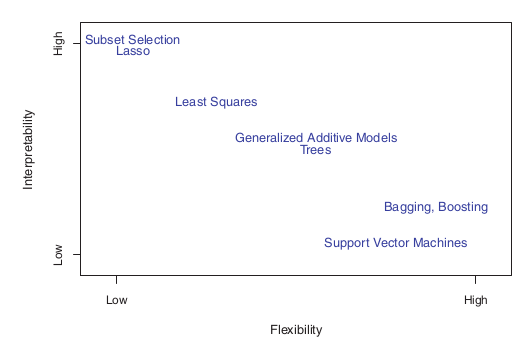
\includegraphics[width=0.75\textwidth]{trade-off_garneth}
  \caption{How the learning algorithms are classified in terms of flexibility vs. interpretability, from ISLR-Gareth \cite{gareth}.}
  \label{}
\end{figure}

\begin{thebibliography}{99}
  \bibitem{gareth}
  Gareth James, Daniela Witten, Trevor Hastie and Robert Tibshirani,
  \textit{Introduction to Statistical Learning with Applications in R},
  Springer,
  2017.

\end{thebibliography}

\end{document}
